\chapter{多元函数微分学}

多元函数微分学与一元函数微分学一样,需要建立导数和微分。

一元函数在工程上基本以时间$t$为自变量,其变化无方向这个概念。
而多元函数不同,它有多个自变量,所以构成的变化量有方向这个概念。
所以多元函数导数讨论的是在一个特定方向上函数的变化率,即方向导数。

而研究与方向相关的变化率较为困难,所以先考察两个自变量方向上的变化率,即偏导。
将一元函数中的导数的概念和定理引入多元函数,再引出全微分,最后引出方向导数和梯度。

本章要点:
\begin{itemize}
    \item 偏导数。
    \item 方向导数。
    \item 全微分。
    \item 梯度。
\end{itemize}

~

\newpage
\section{光滑曲面的第二个要求}

光滑曲面的第二个要求是不折。

这里要捋清几个对应关系。
一元函数对应二维平面,对应{\it xy}直角坐标系,在二维平面中,光滑曲线的要求——不断不折,体现为连续和可导,由于可导和可微的等价性,也可以表现为连续和可微。
二元函数对应三维空间,对应{\it xyz}直角坐标系,在三维空间中,同样对光滑曲面有不折不断的要求,体现为连续和可微,这里的连续和可微都要求各个方向。

定义二元函数的导数是一件麻烦的事情。
首先,二元函数有两个变量,所以变化率会有沿着两个方向。
其次,如果我们考虑一个“总的变化率”,它的大小将随着方向的变化而变化,即总变化率是一个有方向的量,我们用矢量描述它将会比较合适。
综合下来,二元函数中没有“导数”这个概念,与一元函数导数对等的是一个叫“梯度”的概念。
梯度和可微是等价概念。更准确地讲,是一维空间中“导数”这个概念对应着多维空间中的“梯度”和“散度”两个概念。

\begin{table}[h]
\centering
\begin{tabular}{lll}
    \toprule
    概念 & 一元函数中的定义 & 二元函数中的定义\\
    \midrule
    极限        & $\underset{x\rightarrow x_0}{\lim}f\left( x \right) =A$ & $\underset{\boldsymbol{p}\rightarrow \boldsymbol{p}_0}{\lim}f\left( \boldsymbol{p} \right) =A$\\
    连续        & $\underset{x\rightarrow x_0}{\lim}f\left( x \right) =f\left( x_0 \right) $ & $\underset{\boldsymbol{p}\rightarrow \boldsymbol{p}_0}{\lim}f\left( \boldsymbol{p} \right) =f\left( \boldsymbol{p}_0 \right) $\\
    导数/梯度   & $\frac{dy}{dx}$ & $\nabla z=\left( \frac{\partial z}{\partial x}\,\,\frac{\partial z}{\partial y} \right) ^T$\\
    微分/全微分 & $dy=y'dx$ & $dz=\frac{\partial z}{\partial x}dx+\frac{\partial z}{\partial y}dy$\\
    偏导数      &  & $\frac{\partial z}{\partial x},\frac{\partial z}{\partial y}$\\
    方向导数    &  & $\frac{\partial z}{\partial n}=\frac{\partial z}{\partial x}\cos \alpha +\frac{\partial z}{\partial y}\cos \beta $\\
    \bottomrule
\end{tabular}
\end{table}

二元函数中,梯度和全微分都是建立在偏导数的基础上,所以本章先从偏导入手,再介绍全微分和梯度。






\newpage
\section{关于增量的记号}

本节我们先定义一些关于增量的记号。

本节要点:
\begin{itemize}
    \item 熟悉各种增量记号。
\end{itemize}

%============================================================
\subsection{自变量的增量}

\begin{definition}[自变量的增量]
设有一矢量$\boldsymbol{p}$,若它只沿{\it x}轴方向有增量$\Delta x$,此时产生的增量矢称为{\bf $\boldsymbol{p}$沿{\it x}轴方向的偏增量},记作$\Delta _x\boldsymbol{p}$,
同样地,若它只沿{\it y}轴方向有增量$\Delta y$,此时产生的增量矢称为{\bf $\boldsymbol{p}$沿{\it y}轴方向的偏增量},记作$\Delta _y\boldsymbol{p}$,
我们将这个两个偏增量的和称为{\bf 矢量$\boldsymbol{p}$的全增量},记作$\Delta \boldsymbol{p}$,即:
\begin{align*}
&\Delta \boldsymbol{p}=\Delta _x\boldsymbol{p}+\Delta _y\boldsymbol{p}=\Delta x\mathbf{i}+\Delta y\mathbf{j}=\left( \begin{array}{c}
	\Delta x\\
	0\\
\end{array} \right) +\left( \begin{array}{c}
	0\\
	\Delta y\\
\end{array} \right) =\left( \begin{array}{c}
	\Delta x\\
	\Delta y\\
\end{array} \right) \\
&\left\| \Delta \boldsymbol{p} \right\| =\sqrt{\left( \Delta x \right) ^2+\left( \Delta y \right) ^2}
\end{align*}
值得注意的是,$\Delta _x\boldsymbol{p},\Delta _y\boldsymbol{p},\Delta \boldsymbol{p}$依然是矢量。
若有方向$n$,其方向余弦记为$\mathbf{n}=\left( \cos \alpha \,\,\cos \beta \right) ^T$,我们将$\boldsymbol{p}$在方向$n$上的增量称为{\bf $\boldsymbol{p}$沿$n$的方向增量},记作$\Delta _n\boldsymbol{p}$。
\end{definition}

\begin{figure}[h]
\centering
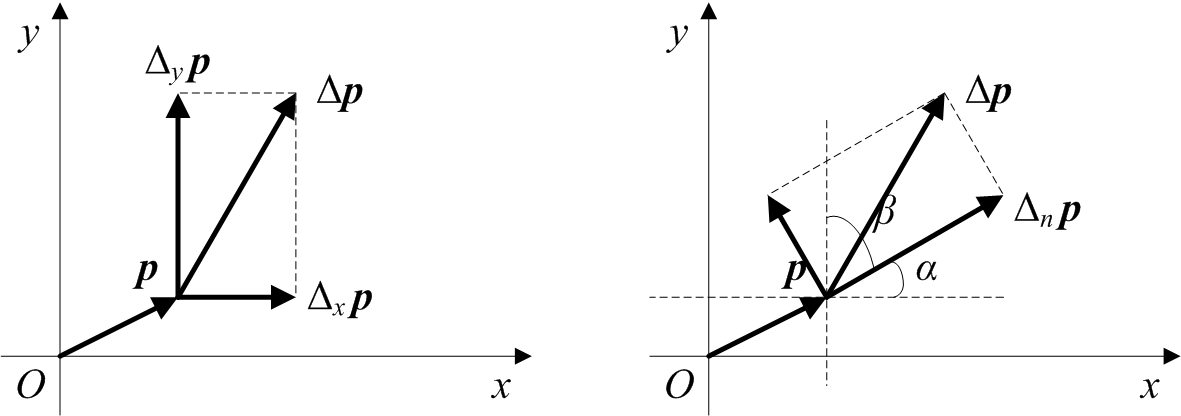
\includegraphics[height=3.5cm]{7.1.png}
\end{figure}

$\Delta _n\boldsymbol{p}$的表达式可以用坐标变换求得。
已知{\it xy}坐标系下的标准基及其构成的矩阵表示$A$:
\[
\boldsymbol{e}_1=\left( \begin{array}{c}
	1\\
	0\\
\end{array} \right) ,\boldsymbol{e}_2=\left( \begin{array}{c}
	0\\
	1\\
\end{array} \right) ,A=\left[ \begin{matrix}
	1&		0\\
	0&		1\\
\end{matrix} \right]
\]
新坐标系为原{\it xy}坐标系逆时针转$\alpha $,可得基及其构成的矩阵表示$W$:
\begin{align*}
&\because \begin{cases}
	L\left( \boldsymbol{e}_1 \right) =\left( \cos \alpha \,\,\sin \alpha \right) ^T\\
	L\left( \boldsymbol{e}_2 \right) =\left( -\sin \alpha \,\,\cos \alpha \right) ^T\\
\end{cases} \\
&\therefore W=\left[ \begin{matrix}
	\cos \alpha&		-\sin \alpha\\
	\sin \alpha&		\cos \alpha\\
\end{matrix} \right]
\end{align*}
由于:
\begin{align*}
&\because \Delta \boldsymbol{p}=A\left( \begin{array}{c}
	\Delta x\\
	\Delta y\\
\end{array} \right) =W\left( \begin{array}{c}
	\Delta n\\
	\Delta n_{\bot}\\
\end{array} \right) \\
&\therefore \left( \begin{array}{c}
	\Delta n\\
	\Delta n_{\bot}\\
\end{array} \right) =W^{-1}A\left( \begin{array}{c}
	\Delta x\\
	\Delta y\\
\end{array} \right) =\left( \begin{array}{c}
	\cos \alpha \Delta x+\sin \alpha \Delta y\\
	-\sin \alpha \Delta x+\cos \alpha \Delta y\\
\end{array} \right) \\
&\therefore \begin{cases}
	\Delta _n\boldsymbol{p}=\left( \begin{array}{c}
	\cos \alpha \Delta x+\sin \alpha \Delta y\\
	0\\
\end{array} \right)\\
	\Delta _{n_{\bot}}\boldsymbol{p}=\left( \begin{array}{c}
	0\\
	-\sin \alpha \Delta x+\cos \alpha \Delta y\\
\end{array} \right)\\
\end{cases}
\end{align*}
$\Delta _n\boldsymbol{p}$在{\it xy}坐标系下的表示:
\begin{align*}
&\because \Delta _n\boldsymbol{p}=A\left[ \Delta _n\boldsymbol{p} \right] _{xy}=W\left[ \Delta _n\boldsymbol{p} \right] _{nn_{\bot}}=W\left( \begin{array}{c}
	\cos \alpha \Delta x+\sin \alpha \Delta y\\
	0\\
\end{array} \right) \\
&\begin{aligned}
	\therefore \left[ \Delta _n\boldsymbol{p} \right] _{xy}&=\left[ \begin{matrix}
	\cos \alpha&		\sin \alpha\\
	-\sin \alpha&		\cos \alpha\\
\end{matrix} \right] \left( \begin{array}{c}
	\cos \alpha \Delta x+\sin \alpha \Delta y\\
	0\\
\end{array} \right)\\
    &=\left( \begin{array}{c}
	\cos \alpha \cos \alpha \Delta x+\sin \alpha \cos \alpha \Delta y\\
	-\sin \alpha \cos \alpha \Delta x-\sin \alpha \sin \alpha \Delta y\\
\end{array} \right)\\
	&=\left[ \begin{matrix}
	\cos \alpha \cos \alpha&		\sin \alpha \cos \alpha\\
	-\sin \alpha \cos \alpha&		-\sin \alpha \sin \alpha\\
\end{matrix} \right] \left( \begin{array}{c}
	\Delta x\\
	\Delta y\\
\end{array} \right)\\
	&=\left[ \begin{matrix}
	\cos \alpha \cos \alpha&		\cos \beta \cos \alpha\\
	-\cos \alpha \cos \beta&		-\cos \beta \cos \beta\\
\end{matrix} \right] \Delta \boldsymbol{p}\\
\end{aligned}
\end{align*}

\begin{tcolorbox}
这里需要重点弄清方向增量和全增量的关系。
\end{tcolorbox}

%============================================================
\subsection{因变量的增量}

\begin{definition}[因变量的增量]
若$z=f\left( \boldsymbol{p} \right) $,设开集$D$中的$\boldsymbol{p}$有偏增量$\Delta _x\boldsymbol{p},\Delta _y\boldsymbol{p}$,此时各自引起的$z$的增量称为{\bf 因变量$z$的偏增量},记为$\Delta _xz,\Delta _yz$,
同样地,若$\boldsymbol{p}$有全增量$\Delta \boldsymbol{p}$,则称引起的$z$的增量为{\bf 因变量$z$的全增量},记作$\Delta z$,
对应地,$\boldsymbol{p}$在$n$方向上的增量引起的$z$的增量称为{\bf 因变量$z$的方向增量},记作$\Delta _nz$,即:
\begin{align*}
&\Delta _xz=f\left( \boldsymbol{p}+\Delta _x\boldsymbol{p} \right) -f\left( \boldsymbol{p} \right) \\
&\Delta _yz=f\left( \boldsymbol{p}+\Delta _y\boldsymbol{p} \right) -f\left( \boldsymbol{p} \right) \\
&\Delta z=f\left( \boldsymbol{p}+\Delta \boldsymbol{p} \right) -f\left( \boldsymbol{p} \right) \\
&\Delta _nz=f\left( \boldsymbol{p}+\Delta _n\boldsymbol{p} \right) -f\left( \boldsymbol{p} \right)
\end{align*}
\end{definition}






\newpage
\section{偏导数和方向导数}

和一元函数一样,二元函数中我们也考察因变量对于自变量的变化率。
我们首先着重在一个维度(一个元)上考察函数的变化率——偏导,该概念用于引出后续的全微分、方向导数、梯度等概念,然后介绍方向导数,关于方向导数更多内容等讨论完全微分后继续深入。
本节着重理解偏导数的概念。

本节要点:
\begin{itemize}
    \item 掌握偏导数的定义;
    \item 了解二阶混偏相等定理;
    \item 了解方向导数的概念。
\end{itemize}

%============================================================
\subsection{偏导数的概念}

\begin{definition}[偏导数]
设函数$z=f\left( \boldsymbol{p} \right) $在点$\boldsymbol{p}_0$的某邻域内有定义,当$\boldsymbol{p}$有偏增量$\Delta _x\boldsymbol{p}$,相应地$z$也有偏增量$\Delta _xz$,如果$\Delta x\rightarrow 0$时,$\Delta _xz/\Delta x$的极限存在,则称此极限为{\bf 函数$z=f\left( \boldsymbol{p} \right) $在$\boldsymbol{p}_0$处对$x$的偏导数},记为$\left. \frac{\partial z}{\partial x} \right|_{\boldsymbol{p}_0}$,即:
\[
\left. \frac{\partial z}{\partial x} \right|_{\boldsymbol{p}_0}:=\underset{\Delta x\rightarrow 0}{\lim}\frac{\Delta _xz}{\Delta x}=\underset{\Delta x\rightarrow 0}{\lim}\frac{f\left( \boldsymbol{p}_0+\Delta _x\boldsymbol{p} \right) -f\left( \boldsymbol{p}_0 \right)}{\Delta x}
\]
也可记为$f_x\left( \boldsymbol{p}_0 \right) $。
同样定义$f_y\left( \boldsymbol{p}_0 \right) $,略。
\end{definition}

需要特别注意的是,偏导数是一个固定的实数。

\begin{definition}[偏导函数]
如果函数$z=f\left( \boldsymbol{p} \right) $在区域$D$内每一点,$\frac{\partial z}{\partial x},\frac{\partial z}{\partial y}
$存在,则称它们为{\bf $z=f\left( \boldsymbol{p} \right) $在区域$D$上的偏导函数},也可记为$f_x\left( \boldsymbol{p} \right) ,f_y\left( \boldsymbol{p} \right) $。
\end{definition}

除非特别指明,一般我们将偏导函数简称为偏导数。
需要特别注意的是,偏导函数依然是一个二元数量值函数。

由于偏导数只考虑一个变量,固定了其余所有变量,即把多元函数“退化”成一元函数,所以本质上偏导数还是一元函数中的导数。
偏导基于偏增量的概念——“固定一个,变动一个”,只要涉及偏导的定理,其证明过程都离不开偏增量概念。

二元函数极限的要求是“任意性”和“唯一性”。
而偏导数是固定了一个变量,变化另一个变化,缺乏了“任意性”,其次,二元函数在某点的各个偏导数不一定相同,缺乏“唯一性”,所以,函数在$\boldsymbol{p}_0$存在偏导数,并不能由此断定在该点存在极限,更不能断定在该点处连续。

%============================================================
\subsection{偏导数的几何意义}

对于二元函数$z=f\left( \boldsymbol{p} \right) $的偏导数$\frac{\partial z}{\partial x}$,由于固定了$y=y_0$,该函数变成了一元函数$z=f\left( x,y_0 \right) $。
几何上,是曲面$z=f\left( \boldsymbol{p} \right) $和平面$y=y_0$的交线。
偏导数的几何意义是曲线$z=f\left( x,y_0 \right) $在点$\boldsymbol{p}_0=\left( x_0\,\,y_0 \right) ^T$处的切线的斜率。

这里要注意,偏导的存在不能说明曲面是不折的,因为偏导相当于将曲面“切片”。
只是说明曲面在这个切片上投影出来的曲线是不折的。

%============================================================
\subsection{高阶偏导数的概念}

\begin{definition}[二阶偏导数]
设函数$z=f\left( \boldsymbol{p} \right) $在区域$D$内的两个偏导数$\frac{\partial z}{\partial x},\frac{\partial z}{\partial y}$都存在,进一步如果它们的偏导数也存在,则称这些偏导数是{\bf $z=f\left( \boldsymbol{p} \right) $的二阶偏导数},记为(二元函数一共4个二阶偏导):
\begin{align*}
&\frac{\partial}{\partial x}\left( \frac{\partial z}{\partial x} \right) =\frac{\partial ^2z}{\partial x^2}=f_{xx}\left( \boldsymbol{p} \right) \\
&\frac{\partial}{\partial y}\left( \frac{\partial z}{\partial x} \right) =\frac{\partial ^2z}{\partial x\partial y}=f_{xy}\left( \boldsymbol{p} \right) \\
&\frac{\partial}{\partial x}\left( \frac{\partial z}{\partial y} \right) =\frac{\partial ^2z}{\partial y\partial x}=f_{yx}\left( \boldsymbol{p} \right) \\
&\frac{\partial}{\partial y}\left( \frac{\partial z}{\partial y} \right) =\frac{\partial ^2z}{\partial y^2}=f_{yy}\left( \boldsymbol{p} \right)
\end{align*}
\end{definition}

\begin{theorem}[二阶混偏相等定理]
设函数$z=f\left( \boldsymbol{p} \right) $的两个二阶混合偏导数$\frac{\partial ^2z}{\partial x\partial y},\frac{\partial ^2z}{\partial y\partial x}$都存在,且这两个二阶混合偏导数都连续,则有
\[
\frac{\partial ^2z}{\partial x\partial y}=\frac{\partial ^2z}{\partial y\partial x}
\]
即:二阶混合偏导存在且均连续则有二阶偏导顺序无关。
\end{theorem}

%============================================================
\subsection{方向导数的概念}

\begin{definition}[方向导数]
设函数$z=f\left( \boldsymbol{p} \right) $在点$\boldsymbol{p}_0$的某邻域内有定义,由该点出发的一个方向$n$,在该方向上$\boldsymbol{p}$有方向增量$\Delta _n\boldsymbol{p}$,进而引起$z$产生方向增量$\Delta _nz$,若当$\left\| \Delta _n\boldsymbol{p} \right\| \rightarrow 0$时,$\frac{\Delta _nz}{\left\| \Delta _n\boldsymbol{p} \right\|}$存在极限,则称此极限为{\bf 函数$z=f\left( \boldsymbol{p} \right) $在点$\boldsymbol{p}_0$处沿方向$n$的方向偏导数},记作 ,即:
\[
\left. \frac{\partial z}{\partial n} \right|_{\boldsymbol{p}_0}:=\lim_{\left\| \Delta _n\boldsymbol{p} \right\| \rightarrow 0} \frac{\Delta _nz}{\left\| \Delta _n\boldsymbol{p} \right\|}=\lim_{\left\| \Delta _n\boldsymbol{p} \right\| \rightarrow 0} \frac{f\left( \boldsymbol{p}_0+\Delta _n\boldsymbol{p} \right) -f\left( \boldsymbol{p}_0 \right)}{\left\| \Delta _n\boldsymbol{p} \right\|}
\]
同样也有{\bf 方向导函数},记作$\frac{\partial z}{\partial n}$。
\end{definition}






\newpage
\section{全微分}

本节讨论全微分。
全微分是多元函数微分学的核心概念,是后续概念和定理的基础,同时在工程上也是一个用于估算微增量的非常有用的概念。

本节要点:
\begin{itemize}
    \item 掌握全微分定义;
    \item 深入理解全微分定理;
    \item 掌握全微分的应用。
\end{itemize}

%============================================================
\subsection{全微分的概念}

\begin{definition}[全微分]
如果区域$D$内有函数$z=f\left( \boldsymbol{p} \right) $,若在$\boldsymbol{p}_0\in D$处全增量满足:
\[
\Delta z=A\left( \boldsymbol{p}_0 \right) \Delta x+B\left( \boldsymbol{p}_0 \right) \Delta y+o\left( \left\| \Delta \boldsymbol{p} \right\| \right)
\]
其中:
\begin{itemize}
    \item $A\left( \boldsymbol{p}_0 \right) ,B\left( \boldsymbol{p}_0 \right) $:只与$\boldsymbol{p}_0$有关、与$\Delta \boldsymbol{p}$无关的常数;
    \item $\left\| \Delta \boldsymbol{p} \right\| $:自变量全增量$\Delta \boldsymbol{p}$的长度;
    \item $o\left( \left\| \Delta \boldsymbol{p} \right\| \right) $:当$\left\| \Delta \boldsymbol{p} \right\| \rightarrow 0$时,关于$\left\| \Delta \boldsymbol{p} \right\| $的高阶无穷小量,
\end{itemize}
则称{\bf 函数$z=f\left( \boldsymbol{p} \right) $在$\boldsymbol{p}_0$处可微},其中,$A\left( \boldsymbol{p}_0 \right) \Delta x+B\left( \boldsymbol{p}_0 \right) \Delta y$称为{\bf 全微分}(也称$\Delta z$的{\bf 线性主部}),记作$dz$,即:
\[
dz:=A\left( \boldsymbol{p}_0 \right) \Delta x+B\left( \boldsymbol{p}_0 \right) \Delta y
\]
如果函数在区域$D$内每点处都可微,则称{\bf 函数$z=f\left( \boldsymbol{p} \right) $在区域$D$内可微},由于$\Delta x=dx,\Delta y=dy$,上式也可写成:
\[
dz=A\left( \boldsymbol{p} \right) dx+B\left( \boldsymbol{p} \right) dy
\]
\end{definition}

%============================================================
\subsection{全微分的代数意义}

全微分表达的意思是,如果全增量$\Delta z$可以分成:
\begin{itemize}
    \item $A\Delta x+B\Delta y$:关于自变量偏增量的一个线性组合;
    \item $o\left( \left\| \Delta \boldsymbol{p} \right\| \right) $:可以忽略的无穷小量,
\end{itemize}
则认为$A\Delta x+B\Delta y$可以代替全增量$\Delta z$,即:
\[
\Delta z=A\Delta x+B\Delta y
\]

\begin{tcolorbox}
“线性化、以直代曲”是微分的目的,无论是多元函数全微分还是一元函数的微分。
\end{tcolorbox}

%============================================================
\subsection{全微分定理}

\begin{theorem}[全微分定理]
函数$z=f\left( \boldsymbol{p} \right) $可微$\Leftrightarrow $函数$z=f\left( \boldsymbol{p} \right) $连续且两个偏导数存在,且$A\left( \boldsymbol{p} \right) =\frac{\partial z}{\partial x},B\left( \boldsymbol{p} \right) =\frac{\partial z}{\partial y}$,即:
\[
dz=\frac{\partial z}{\partial x}dx+\frac{\partial z}{\partial y}dy
\]
\end{theorem}

\begin{proof}
该定理的关键点在于计算偏导$\frac{\partial z}{\partial x}$。
从可微和偏导各自的定义出发:
\begin{align*}
&\Delta z=A\left( \boldsymbol{p}_0 \right) \Delta x+B\left( \boldsymbol{p}_0 \right) \Delta y+o\left( \left\| \Delta \boldsymbol{p} \right\| \right) \\
&\left. \frac{\partial z}{\partial x} \right|_{\boldsymbol{p}_0}=\underset{\Delta x\rightarrow 0}{\lim}\frac{\Delta _xz}{\Delta x}=\underset{\Delta x\rightarrow 0}{\lim}\frac{f\left( \boldsymbol{p}_0+\Delta _x\boldsymbol{p} \right) -f\left( \boldsymbol{p}_0 \right)}{\Delta x}
\end{align*}
计算$\frac{\partial z}{\partial x}$如下:
\begin{align*}
&\left. \frac{\partial z}{\partial x} \right|_{\boldsymbol{p}_0}=\underset{\Delta x\rightarrow 0}{\lim}\frac{\Delta _xz}{\Delta x}=\underset{\Delta x\rightarrow 0}{\lim}\frac{f\left( \boldsymbol{p}_0+\Delta _x\boldsymbol{p} \right) -f\left( \boldsymbol{p}_0 \right)}{\Delta x} \\
&=\underset{\Delta x\rightarrow 0}{\lim}\frac{f\left( \boldsymbol{p}_0+\Delta _x\boldsymbol{p} \right) -f\left( \boldsymbol{p}_0 \right) +f\left( \boldsymbol{p}_0+\Delta \boldsymbol{p} \right) -f\left( \boldsymbol{p}_0+\Delta \boldsymbol{p} \right)}{\Delta x} \\
&=\underset{\Delta x\rightarrow 0}{\lim}\frac{\Delta z+f\left( \boldsymbol{p}_0+\Delta _x\boldsymbol{p} \right) -f\left( \boldsymbol{p}_0+\Delta \boldsymbol{p} \right)}{\Delta x} \\
&=\underset{\Delta x\rightarrow 0}{\lim}\frac{A\left( \boldsymbol{p}_0 \right) \Delta x+B\left( \boldsymbol{p}_0 \right) \Delta y+o\left( \left\| \Delta \boldsymbol{p} \right\| \right) +f\left( \boldsymbol{p}_0+\Delta _x\boldsymbol{p} \right) -f\left( \boldsymbol{p}_0+\Delta \boldsymbol{p} \right)}{\Delta x} \\
&=A\left( \boldsymbol{p}_0 \right) +\underset{\Delta x\rightarrow 0}{\lim}\frac{B\left( \boldsymbol{p}_0 \right) \Delta y-\left[ f\left( \boldsymbol{p}_0+\Delta \boldsymbol{p} \right) -f\left( \boldsymbol{p}_0+\Delta _x\boldsymbol{p} \right) \right] +o\left( \left\| \Delta \boldsymbol{p} \right\| \right)}{\Delta x}
\end{align*}
其中:
\begin{itemize}
    \item $B\left( \boldsymbol{p}_0 \right) \Delta y$:自变量的偏增量$\Delta y$引起的$z$从$\boldsymbol{p}_0$开始的线性部分增量;
    \item $f\left( \boldsymbol{p}_0+\Delta \boldsymbol{p} \right) -f\left( \boldsymbol{p}_0+\Delta _x\boldsymbol{p} \right) $:自变量的偏增量$\Delta y$引起的$z$从$\boldsymbol{p}_0+\Delta _x\boldsymbol{p}$开始的线性部分增量;
    \item $o\left( \left\| \Delta \boldsymbol{p} \right\| \right) $:当$\Delta x\rightarrow 0$时可以忽略的无穷小量。
\end{itemize}
当我们考察$\frac{\partial z}{\partial x}$时,有$\Delta y=0$,所以上述部分中前两部分的值为0,于是上式变为:
\[
\left. \frac{\partial z}{\partial x} \right|_{\boldsymbol{p}_0}=A\left( \boldsymbol{p}_0 \right) +\underset{\Delta x\rightarrow 0}{\lim}\frac{o\left( \left\| \Delta \boldsymbol{p} \right\| \right)}{\Delta x}=A\left( \boldsymbol{p}_0 \right)
\]
\end{proof}

一般函数偏导会存在,但函数本身不一定连续。
连续的前提条件是极限存在。
所以讨论多元函数在某点是否可微,首先得看该函数在该点的是否有极限,再看极限值是否为该函数值,即证明连续。
\begin{align*}
&\text{多元函数:可微} \Leftrightarrow \text{偏导} + \text{连续} \\
&\text{一元函数:可微} \Leftrightarrow \text{偏导} \Rightarrow \text{连续}
\end{align*}

%============================================================
\subsection{函数可微性的讨论}

函数在某点的可微性可从两个思路出发:

一、从微分的定义入手:
\begin{enumerate}
    \item 首先证明函数在该点的偏导数存在;
    \item 再证明余项$o\left( \left\| \Delta \boldsymbol{p} \right\| \right) $为$\left\| \Delta \boldsymbol{p} \right\| $的高阶无穷小量。
\end{enumerate}

二、从全微分定理入手:
\begin{enumerate}
    \item 同上,首先证明函数在该点的偏导数存在;
    \item 再证明函数在该点连续,即证明等式$\underset{\boldsymbol{p}\rightarrow \boldsymbol{p}_0}{\lim}f\left( \boldsymbol{p} \right) =f\left( \boldsymbol{p}_0 \right) $。
\end{enumerate}

~

\begin{example}
设函数$f\left( \boldsymbol{p} \right) =\left| x-y \right|g\left( \boldsymbol{p} \right) $,其中$g\left( \boldsymbol{p} \right) $在原点的某邻域内连续,问为$g\left( \mathbf{0} \right) $何值时$f\left( \boldsymbol{p} \right) $在原点处可微。
\end{example}

解一,从全微分定理入手。

首先考察偏导$f_x\left( \mathbf{0} \right) $对$g\left( \mathbf{0} \right) $的要求。
根据定义:
\[
\left. \frac{\partial f}{\partial x} \right|_{\mathbf{0}}=\underset{x\rightarrow 0}{\lim}\frac{\left| x \right|g\left( x,0 \right) -0\cdot g\left( x,0 \right)}{x-0}=\underset{x\rightarrow 0}{\lim}\frac{\left| x \right|g\left( x,0 \right)}{x}
\]
要使偏导存在,必须该极限存在,即左右极限存在且相等:
\[
\underset{x\rightarrow 0^+}{\lim}\frac{xg\left( x,0 \right)}{x}=\underset{x\rightarrow 0^-}{\lim}\frac{-xg\left( x,0 \right)}{x}
\]
由于$g\left( \boldsymbol{p} \right) $在原点的某邻域内连续,得到$g\left( \mathbf{0} \right) =0$,且有$\left. \frac{\partial f}{\partial x} \right|_{\mathbf{0}}=0$。对$f_y\left( \mathbf{0} \right) $分析,可得到同样结论。
考虑第二个条件——连续,根据定义,需要下式成立:
\[
\underset{x,y\rightarrow 0}{\lim}\left| x-y \right|g\left( x,y \right) =0
\]
由于刚才分析要求$g\left( \mathbf{0} \right) =0$,所以上式必然成立。
综合得到,当$g\left( \mathbf{0} \right) =0$时, 在原点处可微。

解二,从微分的定义出发证明无穷小量,即证明:
\begin{align*}
&\underset{\left\| \Delta \boldsymbol{p} \right\| \rightarrow 0}{\lim}\frac{o\left( \left\| \Delta \boldsymbol{p} \right\| \right)}{\left\| \Delta \boldsymbol{p} \right\|} \\
&=\underset{\left\| \Delta \boldsymbol{p} \right\| \rightarrow 0}{\lim}\frac{\left| \Delta x-\Delta y \right|g\left( \Delta x,\Delta y \right) -0\cdot g\left( 0,0 \right) -\frac{\partial f}{\partial x}\Delta x-\frac{\partial f}{\partial y}\Delta y}{\left\| \Delta \boldsymbol{p} \right\|}
\\
&=\underset{\Delta x,\Delta y\rightarrow 0}{\lim}\frac{\left| \Delta x-\Delta y \right|g\left( \Delta x,\Delta y \right)}{\sqrt{\Delta x^2+\Delta y^2}} \\
&\leqslant \underset{\Delta x,\Delta y\rightarrow 0}{\lim}\frac{\left| \Delta x \right|+\left| \Delta y \right|}{\sqrt{\Delta x^2+\Delta y^2}}g\left( \Delta x,\Delta y \right) \\
&\leqslant \sqrt{2}\cdot \underset{\Delta x,\Delta y\rightarrow 0}{\lim}g\left( \Delta x,\Delta y \right) \\
&=\sqrt{2}\cdot g\left( 0,0 \right) =0
\end{align*}
其中:
\begin{align*}
&\because \frac{\left| \Delta x \right|^2+\left| \Delta y \right|^2+2\left| \Delta x \right|\left| \Delta y \right|}{\left| \Delta x \right|^2+\left| \Delta y \right|^2}\leqslant \frac{\left| \Delta x \right|^2+\left| \Delta y \right|^2+\left| \Delta x \right|^2+\left| \Delta y \right|^2}{\left| \Delta x \right|^2+\left| \Delta y \right|^2}=2 \\
&\therefore \frac{\left| \Delta x \right|+\left| \Delta y \right|}{\sqrt{\left| \Delta x \right|^2+\left| \Delta y \right|^2}}\leqslant \sqrt{2}
\end{align*}

%============================================================
\subsection{全微分的应用——估值及误差}

同一元函数一样,用全微分我们可以近似计算一些工程值,不仅如此,我们还可以知道什么时候能做近似计算,以及误差是多少。
在做估算时,我们用$dz$代替$\Delta z$。
所以估算的关键是:
\begin{itemize}
    \item 构造合适的$f\left( \boldsymbol{p} \right) $,使得偏微分易于计算。
    \item 选定合适的$f\left( \boldsymbol{p}_0 \right) $,使得$\boldsymbol{p}_0$易于计算且对应的$\Delta x,\Delta y$非常小。
\end{itemize}

对于误差分析,我们定义如下概念:
\begin{itemize}
    \item {\bf 真值}:$f\left( \boldsymbol{p}_0+\Delta \boldsymbol{p} \right) $
    \item {\bf 绝对误差}:$\delta _z=\left| f_x\left( \boldsymbol{p}_0 \right) \right|\cdot dx+\left| f_y\left( \boldsymbol{p}_0 \right) \right|\cdot dy$
    \item {\bf 相对误差}:$\frac{\delta _z}{\left| z \right|}=\frac{\left| f_x\left( \boldsymbol{p}_0 \right) \right|\cdot dx+\left| f_y\left( \boldsymbol{p}_0 \right) \right|\cdot dy}{\left| z \right|}$
\end{itemize}

~

\begin{example}
求$1.04^{2.02}$近似值。
\end{example}

解:

首先构造一个合适的函数$z=f\left( \boldsymbol{p} \right) =x^y$,再选定起点$\boldsymbol{p}_0=\left( 1\,\,2 \right) ^T$,得:
\begin{align*}
1.04^{2.02}&\approx f\left( \boldsymbol{p}_0 \right) +dz \\
&=f\left( \boldsymbol{p}_0 \right) +f_x\left( \boldsymbol{p}_0 \right) \cdot dx+f_y\left( \boldsymbol{p}_0 \right) \cdot dy \\
&=1^2+\left. yx^{y-1} \right|_{\boldsymbol{p}_0}\cdot 0.04+\left. x^y\ln x \right|_{\boldsymbol{p}_0}\cdot 0.02 \\
&=1+0.08=1.08
\end{align*}
实际值是1.0824...,还是非常准的。


~

\begin{example}
如果我们通过电压电流测量计算电阻,已知电压表相对误差1\%,电流表相对误差0.5\%,如果测得电阻两端电压和电流分别为32V和8A,分析电阻的误差。
\end{example}

解:

电阻的绝对误差和相对误差:
\begin{align*}
&\delta _R=\left| f_V\left( V,I \right) \right|\cdot dV+\left| f_I\left( V,I \right) \right|\cdot dI=\left| \frac{1}{V} \right|dV+\left| -\frac{V}{I^2} \right|dI \\
&\frac{\delta _R}{\left| R \right|}=\frac{\delta _R}{\left| \frac{V}{I} \right|}
\end{align*}
电压电流的相对误差已知为1\%和0.5\%,可以计算它们的绝对误差:
\begin{align*}
&dV=32\cdot 1\% \\
&dI=8\cdot 0.5\%
\end{align*}
于是:
\begin{align*}
&\delta _R=\left| \frac{1}{V} \right|dV+\left| -\frac{V}{I^2} \right|dI=\frac{1}{8}\cdot \left( 32\cdot 1\% \right) +\frac{32}{8\cdot 8}\cdot \left( 8\cdot 0.5\% \right) =0.06\Omega \\
&\frac{\delta _R}{\left| R \right|}=\frac{\delta _R}{\left| \frac{V}{I} \right|}=\frac{0.06}{\left| \frac{32}{8} \right|}=15\%
\end{align*}






\newpage
\section{多元复合函数的求导}

对于多元复合函数,本节给出链式求导法则。

本节要点:
\begin{itemize}
    \item 掌握链式求导法则;
    \item 掌握引入中间变量转化为复合函数求解非初等多元函数的偏导;
    \item 掌握使用链式求导求解多元函数的高阶偏导;
    \item 了解雅可比矩阵和雅可比行列式。
\end{itemize}

%============================================================
\subsection{多元复合函数的概念}

\begin{definition}[复合函数]
设二元函数$z=z\left( u,v \right) $在某开集$D$有定义,又设$u=u\left( x,y \right) ,v=v\left( x,y \right) $在开集$E$内有定义,于是由$z,u,v$可构成一个{\bf 复合函数}:
\[
z=z\left( u\left( x,y \right) ,v\left( x,y \right) \right) \qquad \left( x,y \right) \in E
\]
\end{definition}

%============================================================
\subsection{多元复合函数的链式求导法则}

\begin{theorem}[链式求导法则]
对于复合函数$z=z\left( u\left( x,y \right) ,v\left( x,y \right) \right) $,若:
\begin{itemize}
    \item $u=u\left( x,y \right) ,v=v\left( x,y \right) $在点$\left( x,y \right) $处偏导存在;
    \item $z=z\left( u,v \right) $对应点$\left( u,v \right) $可微,
\end{itemize}
则$z=z\left( u\left( x,y \right) ,v\left( x,y \right) \right) $在点$\left( x,y \right) $处的偏导数存在,且有链式法则:
\begin{align*}
&\frac{\partial z}{\partial x}=\frac{\partial z}{\partial u}\cdot \frac{\partial u}{\partial x}+\frac{\partial z}{\partial v}\cdot \frac{\partial v}{\partial x} \\
&\frac{\partial z}{\partial y}=\frac{\partial z}{\partial u}\cdot \frac{\partial u}{\partial y}+\frac{\partial z}{\partial v}\cdot \frac{\partial v}{\partial y}
\end{align*}
\end{theorem}

证明略,关键是条件2不能减弱为$z=z\left( u,v \right) $在点$\left( u,v \right) $存在偏导。

~

三种特殊情况。

1、当有三个中间变量时,即$z=z\left( u,v,w \right) $,$u=u\left( x,y \right) $,$v=v\left( x,y \right) $,$w=w\left( x,y \right) $:
\begin{align*}
&\frac{\partial z}{\partial x}=\frac{\partial z}{\partial u}\cdot \frac{\partial u}{\partial x}+\frac{\partial z}{\partial v}\cdot \frac{\partial v}{\partial x}+\frac{\partial z}{\partial w}\cdot \frac{\partial w}{\partial x} \\
&\frac{\partial z}{\partial y}=\frac{\partial z}{\partial u}\cdot \frac{\partial u}{\partial y}+\frac{\partial z}{\partial v}\cdot \frac{\partial v}{\partial y}+\frac{\partial z}{\partial w}\cdot \frac{\partial w}{\partial y}
\end{align*}

2、当只有一个中间变量时,即$z=z\left( u \right) ,u=u\left( x,y \right) $:
\begin{align*}
&\frac{\partial z}{\partial x}=\frac{dz}{du}\cdot \frac{\partial u}{\partial x} \\
&\frac{\partial z}{\partial y}=\frac{dz}{du}\cdot \frac{\partial u}{\partial y}
\end{align*}

3、当只有一个自变量时,即$z=z\left( u,v \right) ,u=u\left( x \right) ,v=v\left( x \right) $,此时的$z$称为{\bf 一元复合函数}:
\[
\frac{dz}{dx}=\frac{\partial z}{\partial u}\cdot \frac{du}{dx}+\frac{\partial z}{\partial v}\cdot \frac{dv}{dx}
\]
该导数称为{\bf $z$对$x$的全导数}。

~

\begin{example}
设$z=\left( x^2+y^2 \right) ^{\sin \left( 2x+y \right)}$,求$\frac{\partial z}{\partial x}$。
\end{example}

解:

对于这类非初等函数,可以引入中间变量,令
\[
\begin{cases}
	u=x^2+y^2\\
	v=\sin \left( 2x+y \right)\\
\end{cases}
\]
则$z=u^v$,有:
\begin{align*}
\frac{\partial z}{\partial x}&=\frac{\partial z}{\partial u}\cdot \frac{\partial u}{\partial x}+\frac{\partial z}{\partial v}\cdot \frac{\partial v}{\partial x} \\
&=vu^{v-1}\cdot 2x+u^v\ln u\cdot 2\cos \left( 2x+y \right) \\
&=2x\cdot \sin \left( 2x+y \right) \cdot \left( x^2+y^2 \right) ^{\sin \left( 2x+y \right) -1} \\
& \quad +2\left( x^2+y^2 \right) ^{\sin \left( 2x+y \right)}\cdot \ln \left( x^2+y^2 \right) \cdot \cos \left( 2x+y \right)
\end{align*}

%============================================================
\subsection{雅可比矩阵和雅可比行列式}

对比一元函数的链式求导,复合函数$y=y\left( u\left( x \right) \right) $对$x$的求导:
\[
\frac{dy}{dx}=\frac{dy}{du}\cdot \frac{du}{dx}
\]
二元函数的链式求导能不能采用这种写法?

考察二元函数的链式求导,二元函数$z=z\left( u\left( x,y \right) ,v\left( x,y \right) \right) $在对$x,y$的偏导数为:
\begin{align*}
&\frac{\partial z}{\partial x}=\frac{\partial z}{\partial u}\cdot \frac{\partial u}{\partial x}+\frac{\partial z}{\partial v}\cdot \frac{\partial v}{\partial x} \\
&\frac{\partial z}{\partial y}=\frac{\partial z}{\partial u}\cdot \frac{\partial u}{\partial y}+\frac{\partial z}{\partial v}\cdot \frac{\partial v}{\partial y}
\end{align*}
采用矩阵方程的形式,可以写成:
\[
\left( \begin{array}{c}
	\frac{\partial z}{\partial x}\\
	\frac{\partial z}{\partial y}\\
\end{array} \right) =\left[ \begin{matrix}
	\frac{\partial u}{\partial x}&		\frac{\partial v}{\partial x}\\
	\frac{\partial u}{\partial y}&		\frac{\partial v}{\partial y}\\
\end{matrix} \right] \left( \begin{array}{c}
	\frac{\partial z}{\partial u}\\
	\frac{\partial z}{\partial v}\\
\end{array} \right)
\]

~

\begin{definition}
我们称由两个二元函数$u\left( x,y \right) ,v\left( x,y \right) $的四个一阶偏导数组成的矩阵称为这两个二元函数的{\bf 雅可比矩阵},即:
\[
\left[ \begin{matrix}
	\frac{\partial u}{\partial x}&		\frac{\partial u}{\partial y}\\
	\frac{\partial v}{\partial x}&		\frac{\partial v}{\partial y}\\
\end{matrix} \right]
\]
其对应的行列式称为{\bf 雅可比行列式},记为$\frac{\partial \left( u,v \right)}{\partial \left( x,y \right)}$,即;
\[
\frac{\partial \left( u,v \right)}{\partial \left( x,y \right)}=\left| \begin{matrix}
	\frac{\partial u}{\partial x}&		\frac{\partial u}{\partial y}\\
	\frac{\partial v}{\partial x}&		\frac{\partial v}{\partial y}\\
\end{matrix} \right|
\]
于是上式可以写为:
\[
\left( \begin{array}{c}
	\frac{\partial z}{\partial x}\\
	\frac{\partial z}{\partial y}\\
\end{array} \right) =\left[ \begin{matrix}
	\frac{\partial u}{\partial x}&		\frac{\partial u}{\partial y}\\
	\frac{\partial v}{\partial x}&		\frac{\partial v}{\partial y}\\
\end{matrix} \right] ^T\left( \begin{array}{c}
	\frac{\partial z}{\partial u}\\
	\frac{\partial z}{\partial v}\\
\end{array} \right)
\]
\end{definition}

同样可扩展三个三元函数$u\left( x,y,z \right) ,v\left( x,y,z \right) ,w\left( x,y,z \right) $的九个一阶偏导数组成的雅可比矩阵:
\[
\left[ \begin{matrix}
	\frac{\partial u}{\partial x}&		\frac{\partial u}{\partial y}&		\frac{\partial u}{\partial z}\\
	\frac{\partial v}{\partial x}&		\frac{\partial v}{\partial y}&		\frac{\partial v}{\partial z}\\
	\frac{\partial w}{\partial x}&		\frac{\partial w}{\partial y}&		\frac{\partial w}{\partial z}\\
\end{matrix} \right]
\]

对于雅可比行列式,有如下法则:
\begin{align*}
&\frac{\partial \left( u,v \right)}{\partial \left( x,y \right)}=\frac{\partial \left( u,v \right)}{\partial \left( s,t \right)}\cdot \frac{\partial \left( s,t \right)}{\partial \left( x,y \right)} \\
&\frac{\partial \left( u,v \right)}{\partial \left( x,y \right)}\cdot \frac{\partial \left( x,y \right)}{\partial \left( u,v \right)}=1 \\
&\frac{\partial \left( u,v \right)}{\partial \left( x,y \right)}=-\frac{\partial \left( v,u \right)}{\partial \left( x,y \right)} \\
&\frac{\partial \left( u,u \right)}{\partial \left( x,y \right)}=0
\end{align*}






\newpage
\section{隐函数的求导}

对于隐函数,本节给出隐函数的求偏导的方法,该方法去除了链式求导步骤,大大简化计算过程。
隐函数求导法在曲线积分和曲面积分中有重要使用,需要熟练掌握。

本节要点:
\begin{itemize}
    \item 掌握一元隐函数和二元隐函数的求导法则。
\end{itemize}

%============================================================
\subsection{一元隐函数的求导}

\begin{theorem}[一元隐函数求导定理]
将方程$F\left( x,y \right) =0$的左边看成二元函数$z=F\left( \boldsymbol{p} \right) $,若满足:
\begin{itemize}
    \item 在点$\boldsymbol{p}_0$的某一邻域内有连续的偏导数,且$\left. \frac{\partial z}{\partial y} \right|_{\boldsymbol{p}_0}\ne 0$,
    \item 点$\boldsymbol{p}_0$满足方程$F\left( \boldsymbol{p}_0 \right) =0$,
\end{itemize}
则点$\boldsymbol{p}_0$的某一邻域内,方程$F\left( x,y \right) =0$将唯一确定单值连续函数$y=y\left( x \right) $,使得$F\left( x,y\left( x \right) \right) =0$,且$y_0=y\left( x_0 \right) $,并有:
\[
\frac{dy}{dx}=-\frac{\frac{\partial z}{\partial x}}{\frac{\partial z}{\partial y}}=-\frac{F_x}{F_y}
\]
\end{theorem}

%============================================================
\subsection{二元隐函数的求导}

\begin{theorem}[二元隐函数求导定理]
将方程$F\left( x,y,z \right) =0$的左边看成三元函数$u=F\left( \boldsymbol{p} \right) ,\boldsymbol{p}=\left( x\,\,y\,\,z \right) ^T$,若满足:
\begin{itemize}
    \item 在点$\boldsymbol{p}_0$的某一邻域内有连续的偏导数,且$\left. \frac{\partial u}{\partial z} \right|_{\boldsymbol{p}_0}\ne 0$,
    \item 点$\boldsymbol{p}_0$满足方程$F\left( \boldsymbol{p}_0 \right) =0$,
\end{itemize}
则点$\boldsymbol{p}_0$的某一邻域内,方程$F\left( x,y,z \right) =0$将唯一确定单值连续函数$z=z\left( x,y \right) $,使得$F\left( x,y,z\left( x,y \right) \right) =0$,且$z_0=z\left( x_0,y_0 \right) $,并有:
\begin{align*}
&\frac{\partial z}{\partial x}=-\frac{\frac{\partial u}{\partial x}}{\frac{\partial u}{\partial z}}=-\frac{F_x}{F_z} \\
&\frac{\partial z}{\partial y}=-\frac{\frac{\partial u}{\partial y}}{\frac{\partial u}{\partial z}}=-\frac{F_y}{F_z}
\end{align*}
\end{theorem}

使用隐函数的求导方法时,首先创建一个函数$u=F\left( \boldsymbol{p} \right) $,此时,$z$再不是应变量,而是自变量。

~

\begin{example}
设$x^2+y^2+z^2=1$,求$\frac{\partial ^2z}{\partial x^2}$。
\end{example}

解:

令$u=F\left( x,y,z \right) =x^2+y^2+z^2-1$,可得:
\[
\frac{\partial z}{\partial x}=-\frac{F_x}{F_z}=-\frac{x}{z}
\]
继续求偏导:
\[
\frac{\partial ^2z}{\partial x^2}=\frac{\partial}{\partial x}\left( -\frac{x}{z} \right) =-\frac{z-x\frac{\partial z}{\partial x}}{z^2}=-\frac{z+x\frac{x}{z}}{z^2}
\]

~

\begin{example}
    设$x^2+y^2+z^2=yf\left( \frac{z}{y} \right) $,其中$f\left( u \right) $对$u$可微,求$\frac{\partial z}{\partial y}$。
\end{example}

解:

令$u=F\left( x,y,z \right) =x^2+y^2+z^2-yf\left( \frac{z}{y} \right) $,可得:
\[
\frac{\partial z}{\partial y}=-\frac{F_y}{F_z}=-\frac{2y-f\left( \frac{z}{y} \right) -yf'\left( \frac{z}{y} \right) \left( -\frac{z}{y^2} \right)}{2z-yf'\left( \frac{z}{y} \right) \frac{1}{y}}=-\frac{2y-f+\frac{z}{y}f'}{2z-f'}
\]

%============================================================
\subsection{方程组的求导}

上面提到的是一个三元方程$F\left( x,y,z \right) =0$确定的一个二元函数。
如果是两个四元方程组成的方程组,如下:
\[
\left\{ \begin{array}{c}
	F\left( x,y,u,v \right) =0\\
	G\left( x,y,u,v \right) =0\\
\end{array} \right.
\]
也可以确定两个二元函数$u=u\left( x,y \right) ,v=v\left( x,y \right) $。
以求$\frac{\partial u}{\partial x},\frac{\partial v}{\partial x}$为例,将两个方程两边分别对$x$求偏导:
\[
\begin{cases}
	\frac{\partial F}{\partial x}+\frac{\partial F}{\partial u}\cdot \frac{\partial u}{\partial x}+\frac{\partial F}{\partial v}\cdot \frac{\partial v}{\partial x}=0\\
	\frac{\partial G}{\partial x}+\frac{\partial G}{\partial u}\cdot \frac{\partial u}{\partial x}+\frac{\partial G}{\partial v}\cdot \frac{\partial v}{\partial x}=0\\
\end{cases}
\]
其实就是解一个二元一次方程组,化为矩阵形式:
\[
\left[ \begin{matrix}
	\frac{\partial F}{\partial u}&		\frac{\partial F}{\partial v}\\
	\frac{\partial G}{\partial u}&		\frac{\partial G}{\partial v}\\
\end{matrix} \right] \cdot \left( \begin{array}{c}
	\frac{\partial u}{\partial x}\\
	\frac{\partial u}{\partial y}\\
\end{array} \right) =-\left( \begin{array}{c}
	\frac{\partial F}{\partial x}\\
	\frac{\partial G}{\partial y}\\
\end{array} \right)
\]
解用雅可比行列式可以写成:
\[
\begin{cases}
	\frac{\partial u}{\partial x}=-\frac{\partial \left( F,G \right)}{\partial \left( x,v \right)}/\frac{\partial \left( F,G \right)}{\partial \left( u,v \right)}\\
	\frac{\partial v}{\partial x}=-\frac{\partial \left( F,G \right)}{\partial \left( u,x \right)}/\frac{\partial \left( F,G \right)}{\partial \left( u,v \right)}\\
\end{cases}
\]

~

\begin{example}
若方程组
\[
\begin{cases}
	u^3+xv-y=0\\
	v^3+yu-x=0\\
\end{cases}
\]
可确定的函数$u=u\left( x,y \right) ,v=v\left( x,y \right) $,求偏导数$\frac{\partial u}{\partial x},\frac{\partial v}{\partial x}$。
\end{example}

解:

用上面的方法,直接写出解的公式:
\begin{align*}
&\frac{\partial \left( F,G \right)}{\partial \left( x,v \right)}=\left| \begin{matrix}
	\frac{\partial F}{\partial x}&		\frac{\partial F}{\partial v}\\
	\frac{\partial G}{\partial x}&		\frac{\partial G}{\partial v}\\
\end{matrix} \right|=v\cdot 3v^2-x\cdot \left( -1 \right) =x+3v^3 \\
&\frac{\partial \left( F,G \right)}{\partial \left( u,x \right)}=\left| \begin{matrix}
	\frac{\partial F}{\partial u}&		\frac{\partial F}{\partial x}\\
	\frac{\partial G}{\partial u}&		\frac{\partial G}{\partial x}\\
\end{matrix} \right|=3u^2\cdot \left( -1 \right) -v\cdot y=-vy-3u^2 \\
&\frac{\partial \left( F,G \right)}{\partial \left( u,v \right)}=\left| \begin{matrix}
	\frac{\partial F}{\partial u}&		\frac{\partial F}{\partial v}\\
	\frac{\partial G}{\partial u}&		\frac{\partial G}{\partial v}\\
\end{matrix} \right|=3u^2\cdot 3v^2-x\cdot y=9u^2v^2-xy
\end{align*}
解得:
\[
\begin{cases}
	\frac{\partial u}{\partial x}=-\frac{\partial \left( F,G \right)}{\partial \left( x,v \right)}/\frac{\partial \left( F,G \right)}{\partial \left( u,v \right)}=-\frac{x+3v^3}{9u^2v^2-xy}\\
	\frac{\partial v}{\partial x}=-\frac{\partial \left( F,G \right)}{\partial \left( u,x \right)}/\frac{\partial \left( F,G \right)}{\partial \left( u,v \right)}=-\frac{-vy-3u^2}{9u^2v^2-xy}\\
\end{cases}
\]



\newpage
\section{全微分的几何意义}

本节是对矢量、全微分和隐函数求导的汇总型应用,是空间矢量和微分的第一次结合,熟练掌握和细品。

本节要点:
\begin{itemize}
    \item 深入理解全微分的几何意义;
    \item 深入理解方向导数的概念。
\end{itemize}

%============================================================
\subsection{空间曲线的切线和法平面}

\begin{figure}[h]
\centering
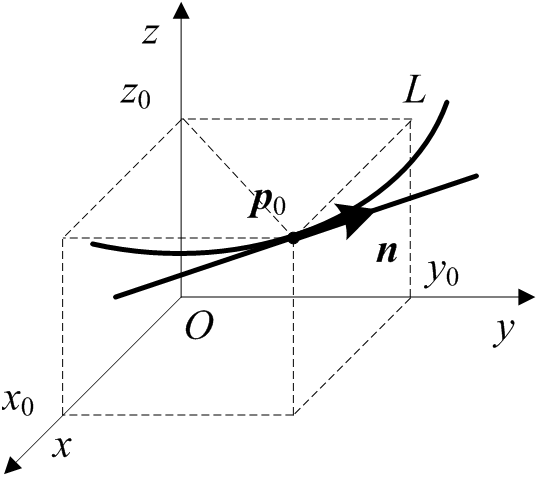
\includegraphics[height=4cm]{7.2.png}
\end{figure}

\begin{definition}
设三维空间的曲线
\[
L:\left\{ \begin{array}{c}
	x=x\left( t \right)\\
	y=y\left( t \right)\\
	z=z\left( t \right)\\
\end{array} \right.
\]
则曲线在点$\boldsymbol{p}_0$处(即对应$t_0$)的切线的方向称为{\bf 曲线$L$的切向量},假设记为$\boldsymbol{n}$,则有:
\[
\boldsymbol{n}=\left. \left( \begin{array}{c}
	x'\\
	y'\\
	z'\\
\end{array} \right) \right|_{t=t_0}=\left( \begin{array}{c}
	x'\left( t_0 \right)\\
	y'\left( t_0 \right)\\
	z'\left( t_0 \right)\\
\end{array} \right)
\]
于是,曲线$L$在点$\boldsymbol{p}_0$处的切线方程为$\boldsymbol{p}-\boldsymbol{p}_0=\lambda \boldsymbol{n}$,展开后为:
\[
\left( \begin{array}{c}
	x\\
	y\\
	z\\
\end{array} \right) -\left( \begin{array}{c}
	x_0\\
	y_0\\
	z_0\\
\end{array} \right) =\lambda \left( \begin{array}{c}
	x'\left( t_0 \right)\\
	y'\left( t_0 \right)\\
	z'\left( t_0 \right)\\
\end{array} \right) \quad \text{或} \quad \frac{x-x_0}{x'\left( t_0 \right)}=\frac{y-y_0}{y'\left( t_0 \right)}=\frac{z-z_0}{z'\left( t_0 \right)}
\]
过点$\boldsymbol{p}_0$垂直于该点切线的平面称为{\bf 曲线$L$在点$\boldsymbol{p}_0$处的法平面},法平面方程为$\left( \boldsymbol{p}-\boldsymbol{p}_0 \right) ^T\boldsymbol{n}=0$,展开后为:
\[
\left( x-x_0 \right) \cdot x'\left( t_0 \right) +\left( y-y_0 \right) \cdot y'\left( t_0 \right) +\left( z-z_0 \right) \cdot z'\left( t_0 \right) =0
\]
\end{definition}

如果曲线由两个平面
\[
L:\left\{ \begin{array}{c}
	F\left( x,y,z \right) =0\\
	G\left( x,y,z \right) =0\\
\end{array} \right.
\]
相交而成,则在点$\boldsymbol{p}_0$处的切向量为:
\[
\boldsymbol{n}=\left. \left( 1\,\,\frac{\partial y}{\partial x}\,\,\frac{\partial z}{\partial x} \right) ^T \right|_{\boldsymbol{p}_0}
\]
切线方程为:
\[
\frac{x-x_0}{1}=\frac{y-y_0}{\left. \frac{\partial y}{\partial x} \right|_{\boldsymbol{p}_0}}=\frac{z-z_0}{\left. \frac{\partial z}{\partial x} \right|_{\boldsymbol{p}_0}}
\]
法平面方程为:
\[
\left( x-x_0 \right) +\left( y-y_0 \right) \cdot \left. \frac{\partial y}{\partial x} \right|_{\boldsymbol{p}_0}+\left( z-z_0 \right) \cdot \left. \frac{\partial z}{\partial x} \right|_{\boldsymbol{p}_0}=0
\]

%============================================================
\subsection{空间曲面的切平面和法线}

\begin{figure}[h]
\centering
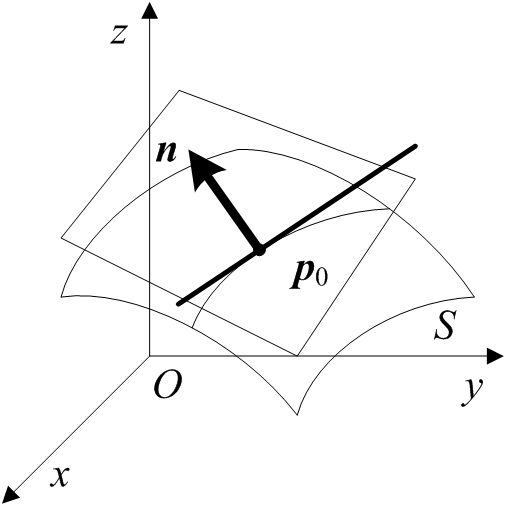
\includegraphics[height=4cm]{7.3.png}
\end{figure}

\begin{definition}
若曲面$S$由方程$F\left( \boldsymbol{p} \right) =0,\boldsymbol{p}=\left( x\,\,y\,\,z \right) ^T$隐式给出,对于在点$\boldsymbol{p}_0$处垂直于切平面的方向称为{\bf 曲面$S$在$\boldsymbol{p}_0$处的法向量},假设记为$\boldsymbol{n}$,则有:
\[
\boldsymbol{n}=\left. \left( \begin{array}{c}
	F_x\\
	F_y\\
	F_z\\
\end{array} \right) \right|_{\boldsymbol{p}_0}
\]
{\bf 曲面$S$在点$\boldsymbol{p}_0$处的法线方程}为$\boldsymbol{p}-\boldsymbol{p}_0=\lambda \boldsymbol{n}$,即:
\[
\left( \begin{array}{c}
	x\\
	y\\
	z\\
\end{array} \right) -\left( \begin{array}{c}
	x_0\\
	y_0\\
	z_0\\
\end{array} \right) =\lambda \left( \begin{array}{c}
	F_x\left( \boldsymbol{p}_0 \right)\\
	F_y\left( \boldsymbol{p}_0 \right)\\
	F_z\left( \boldsymbol{p}_0 \right)\\
\end{array} \right) \quad \text{或} \quad \frac{x-x_0}{F_x\left( \boldsymbol{p}_0 \right)}=\frac{y-y_0}{F_y\left( \boldsymbol{p}_0 \right)}=\frac{z-z_0}{F_z\left( \boldsymbol{p}_0 \right)}
\]
{\bf 曲面$S$在点$\boldsymbol{p}_0$处的切平面方程}为$\left( \boldsymbol{p}-\boldsymbol{p}_0 \right) ^T\boldsymbol{n}=0$,即:
\[
\left( x-x_0 \right) \cdot F_x\left( \boldsymbol{p}_0 \right) +\left( y-y_0 \right) \cdot F_y\left( \boldsymbol{p}_0 \right) +\left( z-z_0 \right) \cdot F_z\left( \boldsymbol{p}_0 \right) =0
\]
\end{definition}

若曲面由$z=z\left( x,y \right) $显式给出,则法向量:
\[
\boldsymbol{n}=\left. \left( \begin{array}{c}
	-z_x\\
	-z_y\\
	1\\
\end{array} \right) \right|_{\boldsymbol{p}_0}
\]
法线方程:
\[
\frac{x-x_0}{-z_x\left( \boldsymbol{p}_0 \right)}=\frac{y-y_0}{-z_y\left( \boldsymbol{p}_0 \right)}=\frac{z-z_0}{1}
\]
切平面方程:
\[
-\left( x-x_0 \right) \cdot z_x\left( \boldsymbol{p}_0 \right) -\left( y-y_0 \right) \cdot z_y\left( \boldsymbol{p}_0 \right) +\left( z-z_0 \right) =0
\]

~

\begin{example}
求曲面$x^2+2y^2+3z^2=6$在$\boldsymbol{p}_0=\left( 1\,\,1\,\,1 \right) $处的切平面和法线。
\end{example}

解:

构造$F=x^2+2y^2+3z^2-6$,得$\boldsymbol{p}_0$处的法线方向:
\[
\boldsymbol{n}=\left. \left( \begin{array}{c}
	F_x\\
	F_y\\
	F_z\\
\end{array} \right) \right|_{\boldsymbol{p}_0}=\left. \left( \begin{array}{c}
	2x\\
	4y\\
	6z\\
\end{array} \right) \right|_{\boldsymbol{p}_0}=\left( \begin{array}{c}
	2\\
	4\\
	6\\
\end{array} \right)
\]
切平面和法线:
\begin{align*}
&2\left( x-1 \right) +4\left( y-1 \right) +6\left( z-1 \right) =0 \\
&\frac{x-1}{2}=\frac{y-1}{4}=\frac{z-1}{6}
\end{align*}

%============================================================
\subsection{全微分的几何意义}

根据上节的空间曲面$z=z\left( x,y \right) $的切平面方程,对比全微分,如下:
\begin{align*}
&-\left( x-x_0 \right) \cdot z_x\left( \boldsymbol{p}_0 \right) -\left( y-y_0 \right) \cdot z_y\left( \boldsymbol{p}_0 \right) +\left( z-z_0 \right) =0 \\
&dz=z_x\cdot dx+z_y\cdot dy
\end{align*}
$z=z\left( x,y \right) $在点$\boldsymbol{p}_0$处的全微分的几何意义表示曲面$S$在点$\boldsymbol{p}_0$处的切平面在{\it z}轴的增量。

全微分的几何意义体现出一点,曲面要在某一点有切平面,必须在这一点光滑——不断不折。
只有光滑了,才有切平面,才有切平面在{\it z}轴的增量。
细品!

%============================================================
\subsection{方向导数定理}

我们之前定义了方向导数
\[
\left. \frac{\partial z}{\partial n} \right|_{\boldsymbol{p}_0}=\underset{\left\| \Delta _n\boldsymbol{p} \right\| \rightarrow 0}{\lim}\frac{\Delta _nz}{\left\| \Delta _n\boldsymbol{p} \right\|}=\underset{\left\| \Delta _n\boldsymbol{p} \right\| \rightarrow 0}{\lim}\frac{f\left( \boldsymbol{p}_0+\Delta _n\boldsymbol{p} \right) -f\left( \boldsymbol{p}_0 \right)}{\left\| \Delta _n\boldsymbol{p} \right\|}
\]
但当时还没有引入全微分,我们这里用全微分完善方向导数。

\begin{theorem}[方向导数定理]
设函数$z=z\left( \boldsymbol{p} \right) $在一点处可微,则该函数在此点处存在沿任意方向$n$的方向导数,且有:
\[
\frac{\partial z}{\partial n}=\frac{\partial z}{\partial x}\cos \alpha +\frac{\partial z}{\partial y}\cos \beta
\]
其中,$\mathbf{n}=\left( \cos \alpha \,\,\cos \beta \right) ^T$为方向$n$的方向余弦。
\end{theorem}

该定理给方向导数的计算提供了方法,即如果知道一个方向,就能知道沿该方向的方向导数。

同样,对于三元函数$u=u\left( \boldsymbol{p} \right) ,\boldsymbol{p}\in \mathbb{R} ^3$,方向导数为:
\[
\frac{\partial u}{\partial n}=\frac{\partial u}{\partial x}\cos \alpha +\frac{\partial u}{\partial y}\cos \beta +\frac{\partial u}{\partial z}\cos \gamma
\]

~

\begin{example}
求函数$z=xe^{2y}$在点$\boldsymbol{p}_0=\left( 1\,\,0 \right) ^T$处,沿射线$\left( 1\,\,0 \right) ^T\rightarrow \left( 2\,\,-1 \right) ^T$的方向导数。
\end{example}

解:

首先求得偏导:
\[
\left. \left( \frac{\partial z}{\partial x}\,\,\frac{\partial z}{\partial y} \right) ^T \right|_{\boldsymbol{p}_0}=\left. \left( e^{2y} \quad 2xe^{2y} \right) ^T \right|_{\boldsymbol{p}_0}=\left( 1\,\,2 \right) ^T
\]
再求射线的方向余弦:
\begin{align*}
&\because \Delta _n\boldsymbol{p}=\left( \begin{array}{c}
	2\\
	-1\\
\end{array} \right) -\left( \begin{array}{c}
	1\\
	0\\
\end{array} \right) =\left( \begin{array}{c}
	1\\
	-1\\
\end{array} \right)
\\
&\therefore \left\| \Delta _n\boldsymbol{p} \right\| =\sqrt{2} \\
&\therefore \mathbf{\theta }=\left( \frac{1}{\sqrt{2}}\,\,\frac{-1}{\sqrt{2}} \right) ^T
\end{align*}
最终,方向导数:
\[
\left. \frac{\partial z}{\partial n} \right|_{\boldsymbol{p}_0}=\left( 1\,\,2 \right) \left( \frac{1}{\sqrt{2}}\,\,\frac{-1}{\sqrt{2}} \right) ^T=\frac{1}{\sqrt{2}}+\frac{-2}{\sqrt{2}}=-\frac{1}{\sqrt{2}}
\]






\newpage
\section{梯度}

通过方向导数我们可以看到,若一个函数可微则任何方向的导数可以分解为两个偏导的线性组合,于是偏导可以认为是一个坐标系。
本节将这个概念定义化。

本节要点:
\begin{itemize}
    \item 掌握梯度的概念;
    \item 理解梯度的几何意义;
    \item 理解微分算子的概念。
\end{itemize}

%============================================================
\subsection{梯度的概念}

\begin{definition}[梯度]
设函数$z=z\left( \boldsymbol{p} \right) $在一点处可微,则称其两个偏导构成的矢量$\left( \frac{\partial z}{\partial x}\,\,\frac{\partial z}{\partial y} \right) ^T$为{\bf $z=z\left( \boldsymbol{p} \right) $在该点处的梯度},记为$\mathbf{grad}z$,简记为$\nabla z$,即:
\[
\nabla z:=\left( \begin{array}{c}
	\frac{\partial z}{\partial x}\\
	\frac{\partial z}{\partial y}\\
\end{array} \right)
\]
\end{definition}

梯度的特点:
\begin{itemize}
    \item 梯度是一个矢量,由对各个坐标的偏导构成;
    \item 梯度的方向就是最大的方向导数的方向;
    \item 梯度的模就是最大的方向导数的值。
\end{itemize}

于是,我们可以用梯度描述方向导数,如下:
\[
\frac{\partial z}{\partial n}=\frac{\partial z}{\partial x}\cos \alpha +\frac{\partial z}{\partial y}\cos \beta =\nabla z^T\mathbf{n}=\left\| \nabla z \right\| \cos \theta
\]
其中,
\begin{itemize}
    \item $\mathbf{n}=\left( \cos \alpha \,\,\cos \beta \right) ^T$:方向$n$的方向余弦;
    \item $\theta $:方向$n$和梯度的夹角。
\end{itemize}

\begin{figure}[h]
\centering
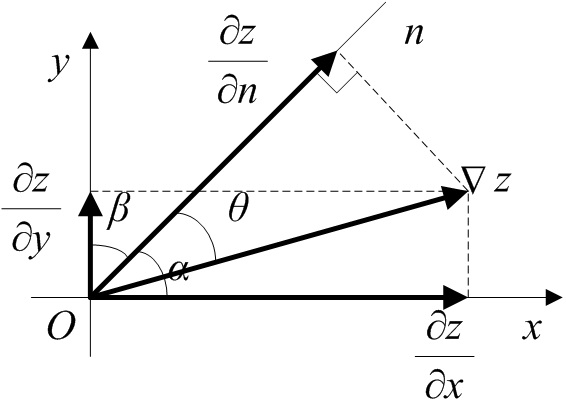
\includegraphics[height=3.5cm]{7.4.png}
\end{figure}

%============================================================
\subsection{梯度的几何意义}

几何上,梯度与等值线有垂直关系。
以二维平面的数量场为例,点$\boldsymbol{p}_0$的梯度:
\begin{itemize}
    \item 方向是等值线上该点的法向方向;
    \item 大小是$\left. \left\| \nabla z \right\| \right|_{\boldsymbol{p}_0}$。
\end{itemize}

\begin{figure}[h]
\centering
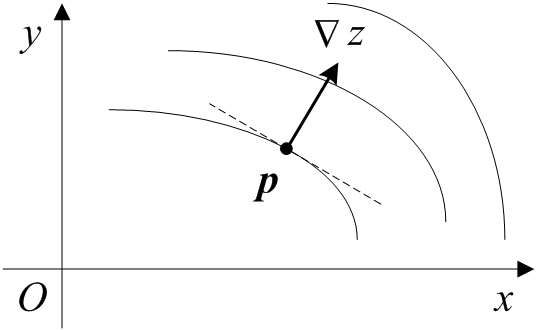
\includegraphics[height=3cm]{7.5.png}
\end{figure}

%============================================================
\subsection{梯度的物理意义}

物理上任何一个数量场,只要有变化(无变化也可以)都会有变化率,变化率可以分解到{\it xy}坐标,构成一个矢量。
所以,只有数量场才有梯度,是一个描述数量场的变化率的矢量场,其次梯度是由数量场决定的,可以认为是该数量场的性质。

%============================================================
\subsection{向量微分算子}

从纯粹的数学上,可以再进一步把“计算梯度”这一数学计算抽象出来,写成记号:
\[
\nabla :=\left( \begin{array}{c}
	\frac{\partial}{\partial x}\\
	\frac{\partial}{\partial y}\\
\end{array} \right)
\]
称为{\bf 向量微分算子},又称{\bf 哈密尔顿算子}:
\begin{itemize}
    \item 首先,它是一个算子,是纯数学上的一个计算符号,本身不承载任何物理意义;
    \item 其次是一个进行微分运算的算子;
    \item 最后是向量,表示这个微分算子是对构成其目标对象的基的微分运算,结果是一个矢量。
\end{itemize}
于是,梯度可以理解为微分算子和数量场的积,或者更简单的是“一个矢量的数乘”:
\[
\nabla z=\left( \begin{array}{c}
	\frac{\partial}{\partial x}\\
	\frac{\partial}{\partial y}\\
\end{array} \right) z=\left( \begin{array}{c}
	\frac{\partial z}{\partial x}\\
	\frac{\partial z}{\partial y}\\
\end{array} \right)
\]

~

梯度的运算法则:
\begin{align*}
&\nabla Cf=C\nabla f \\
&\nabla \left( f+g \right) =\nabla f+\nabla g \\
&\nabla \left( fg \right) =g\nabla f+f\nabla g \\
&\nabla f\left( u \right) =\frac{df}{du}\nabla u
\end{align*}






\newpage
\section{二元函数的泰勒展开}

之前在一元函数中,我们讨论了泰勒展开,这里我们进一步讨论二元函数的泰勒展开。

本节要点:
\begin{itemize}
    \item 掌握二元函数的泰勒展开;
    \item 了解黑塞矩阵。
\end{itemize}

%============================================================
\subsection{二元函数的泰勒展开}

\begin{theorem}[泰勒定理(拉格朗日型)]
若函数$f\left( x,y \right) $在$\left( x_0,y_0 \right) $的某邻域$N$内具有n+1阶连续偏导数,$\left( x_0+h,y_0+k \right) \in N$,则有:
\begin{align*}
f\left( x_0+h,y_0+k \right) =&f\left( x_0,y_0 \right) + \\
&\left( h\frac{\partial}{\partial x}+k\frac{\partial}{\partial y} \right) f\left( x_0,y_0 \right) + \\
&\frac{1}{2!}\left( h\frac{\partial}{\partial x}+k\frac{\partial}{\partial y} \right) ^2f\left( x_0,y_0 \right) + \\
&\cdots \\
&\frac{1}{n!}\left( h\frac{\partial}{\partial x}+k\frac{\partial}{\partial y} \right) ^nf\left( x_0,y_0 \right) + \\
&R_n
\end{align*}
其中:
\begin{itemize}
    \item $R_n=\frac{1}{\left( n+1 \right) !}\left( h\frac{\partial}{\partial x}+k\frac{\partial}{\partial y} \right) ^{n+1}f\left( x_0+\theta h,y_0+\theta k \right) ,\theta \in \left( 0,1 \right) $:{\bf 拉格朗日余项};
\end{itemize}
该展开称为{\bf $f\left( x,y \right) $在$\left( x_0,y_0 \right) $的$n$阶具有拉格朗日余项的泰勒公式}。
上式中的记号:
\begin{align*}
&\left( h\frac{\partial}{\partial x}+k\frac{\partial}{\partial y} \right) f\left( x_0,y_0 \right) =hf_x\left( x_0,y_0 \right) +kf_y\left( x_0,y_0 \right) \\
&\left( h\frac{\partial}{\partial x}+k\frac{\partial}{\partial y} \right) ^2f\left( x_0,y_0 \right) =h^2f_{xx}\left( x_0,y_0 \right) +2hkf_{xy}\left( x_0,y_0 \right) +k^2f_{yy}\left( x_0,y_0 \right) \\
&\left( h\frac{\partial}{\partial x}+k\frac{\partial}{\partial y} \right) ^nf\left( x_0,y_0 \right) =\sum_{i=0}^n{\left[ C_{n}^{i}h^ik^{n-i}\frac{\partial ^nf\left( x_0,y_0 \right)}{\partial x^i\partial y^{n-i}} \right]}
\end{align*}
\end{theorem}

证明略,大致是一元泰勒展开+复合函数的链式求导,详见“教材\cite{book1}”。

\begin{theorem}[泰勒定理(佩亚诺型)]
若函数$f\left( x,y \right) $在$\left( x_0,y_0 \right) $的某邻域$N$内具有n阶连续偏导数,$\left( x_0+h,y_0+k \right) \in N$,则有:
\begin{align*}
f\left( x_0+h,y_0+k \right) =&f\left( x_0,y_0 \right) + \\
&\left( h\frac{\partial}{\partial x}+k\frac{\partial}{\partial y} \right) f\left( x_0,y_0 \right) + \\
&\frac{1}{2!}\left( h\frac{\partial}{\partial x}+k\frac{\partial}{\partial y} \right) ^2f\left( x_0,y_0 \right) + \\
&\cdots \\
&\frac{1}{n!}\left( h\frac{\partial}{\partial x}+k\frac{\partial}{\partial y} \right) ^nf\left( x_0,y_0 \right) + \\
&o\left( \rho ^n \right)
\end{align*}
其中:
\begin{itemize}
    \item $\rho =\sqrt{h^2+k^2}$:{\bf 佩亚诺余项};
\end{itemize}
该展开称为{\bf $f\left( x,y \right) $在$\left( x_0,y_0 \right) $的$n$阶具有佩亚诺余项的泰勒公式}。
\end{theorem}

%============================================================
\subsection{黑塞Hessian矩阵}

当我们考虑二阶拉格朗日余项的泰勒展开:
\begin{align*}
f\left( x_0+h,y_0+k \right) =&f\left( x_0,y_0 \right) + \\
&\left( h\frac{\partial}{\partial x}+k\frac{\partial}{\partial y} \right) f\left( x_0,y_0 \right) + \\
&\frac{1}{2!}\left( h\frac{\partial}{\partial x}+k\frac{\partial}{\partial y} \right) ^2f\left( x_0,y_0 \right) + \\
&R_3
\end{align*}
其中,第二项写成向量形式:
\[
\left( h\frac{\partial}{\partial x}+k\frac{\partial}{\partial y} \right) f\left( x_0,y_0 \right) =\left( \begin{array}{c}
	h\\
	k\\
\end{array} \right) ^T\left( \begin{array}{c}
	\left. \frac{\partial f}{\partial x} \right|_{\boldsymbol{p}_0}\\
	\left. \frac{\partial f}{\partial y} \right|_{\boldsymbol{p}_0}\\
\end{array} \right) =\left( \begin{array}{c}
	h\\
	k\\
\end{array} \right) ^T\nabla f_{\boldsymbol{p}_0}
\]
第三项写成向量形式:
\begin{align*}
\left( h\frac{\partial}{\partial x}+k\frac{\partial}{\partial y} \right) ^2f\left( x_0,y_0 \right) &=h^2f_{xx}\left( \boldsymbol{p}_0 \right) +2hkf_{xy}\left( \boldsymbol{p}_0 \right) +k^2f_{yy}\left( \boldsymbol{p}_0 \right) \\
&=\left( \begin{array}{c}
	h\\
	k\\
\end{array} \right) ^T\left[ \begin{matrix}
	\left. f_{xx} \right|_{\boldsymbol{p}_0}&		\left. f_{xy} \right|_{\boldsymbol{p}_0}\\
	\left. f_{yx} \right|_{\boldsymbol{p}_0}&		\left. f_{yy} \right|_{\boldsymbol{p}_0}\\
\end{matrix} \right] \left( \begin{array}{c}
	h\\
	k\\
\end{array} \right)
\end{align*}
我们将矩阵
\[
H_f=\left[ \begin{matrix}
	f_{xx}&		f_{xy}\\
	f_{yx}&		f_{yy}\\
\end{matrix} \right]
\]
称为{\bf 函数$f\left( x,y \right) $的黑塞(Hessian)矩阵},记作$H_f$,特别地,当$f\left( x,y \right) $具有二阶连续偏导时,有$f_{xy}=f_{yx}$,于是Hessian矩阵为对称矩阵,即$H_f={H_f}^T$。

于是,二阶拉格朗日余项的泰勒展开用矩阵形式可以写成矩阵形式:
\begin{align*}
f\left( \boldsymbol{p} \right) =&f\left( \boldsymbol{p}_0 \right) + \\
&\left( \boldsymbol{p}-\boldsymbol{p}_0 \right) ^T\nabla f_{\boldsymbol{p}_0}+ \\
&\frac{1}{2!}\left( \boldsymbol{p}-\boldsymbol{p}_0 \right) ^TH_f\left( \boldsymbol{p}_0 \right) \left( \boldsymbol{p}-\boldsymbol{p}_0 \right) + \\
&R_3
\end{align*}

一元函数是标量,所以其一阶导数和二阶导数都是标量。
二元函数虽然是标量,但一阶导数(也即梯度)就是一个矢量,二阶导数就是一个$2\times 2$矩阵,这就是黑塞矩阵。
所以黑塞矩阵相当于一元函数中的二阶导数,可用于判断函数的极值。






\newpage
\section{多元函数的极值}

之前在一元函数中我们用导数讨论了极值问题,这里我们扩展到二元函数,用梯度和黑塞矩阵讨论二元函数的极值问题。

本节要点:
\begin{itemize}
    \item 掌握二元函数的极值的概念;
    \item 深刻理解二元函数极值的判断方法;
    \item 了解条件极值和拉格朗日乘数法。
\end{itemize}

%============================================================
\subsection{极值的概念}

\begin{definition}[极值]
若函数$f\left( \boldsymbol{p} \right) $在点$\boldsymbol{p}_0$的某去心邻域$N\left( \boldsymbol{\hat{p}}_0,\delta \right) $内任意一点$\boldsymbol{p}$有
\[
f\left( \boldsymbol{p} \right) >f\left( \boldsymbol{p}_0 \right) \quad \text{或} \quad f\left( \boldsymbol{p} \right) <f\left( \boldsymbol{p}_0 \right)
\]
则称$f\left( \boldsymbol{p}_0 \right) $为{\bf 函数$f\left( \boldsymbol{p} \right) $的极小值}(或{\bf 极大值}),点$\boldsymbol{p}_0$为{\bf 函数的极小值点}(或{\bf 极大值点})。
我们统称极小值和极大值为{\bf 极值},极小值点和极大值点为{\bf 极值点}。
\end{definition}

在讨论函数$f\left( \boldsymbol{p} \right) $的极值问题时,我们将$f\left( \boldsymbol{p} \right) $称为{\bf 目标函数},这类问题称为无条件极值问题。
如果加了一些限定条件如$g\left( \boldsymbol{p} \right) =0$(也可以是不等式),则称为{\bf 条件极值}。

%============================================================
\subsection{极值的判断}

类似于一元函数,二元函数的极值判断也有充分条件和必要条件。

\begin{theorem}[极值的充分条件]
若函数$f\left( \boldsymbol{p} \right) $在$\boldsymbol{p}_0$处有偏导,在$\boldsymbol{p}_0$取得极值,则:
\[
f_x\left( \boldsymbol{p}_0 \right) =f_y\left( \boldsymbol{p}_0 \right) =0
\]
用矢量写为:
\[
\nabla f\left( \boldsymbol{p}_0 \right) =\mathbf{0}
\]
符合上式的$\boldsymbol{p}_0$称为{\bf 函数的驻点}。
\end{theorem}

\begin{theorem}[极值的必要条件]
若函数$f\left( \boldsymbol{p} \right) $在$\boldsymbol{p}_0$的某邻域内有二阶连续偏导,且$f_x\left( \boldsymbol{p}_0 \right) =f_y\left( \boldsymbol{p}_0 \right) =0$,记函数$f\left( \boldsymbol{p} \right) $在$\boldsymbol{p}_0$的黑塞矩阵
\[
H_f\left( \boldsymbol{p}_0 \right) =\left. \left[ \begin{matrix}
	f_{xx}&		f_{xy}\\
	f_{yx}&		f_{yy}\\
\end{matrix} \right] \right|_{\boldsymbol{p}_0}\triangleq \left[ \begin{matrix}
	A&		B\\
	B&		C\\
\end{matrix} \right]
\]
\begin{itemize}
    \item 当$H_f\left( \boldsymbol{p}_0 \right) $为正定矩阵,即$AC>B^2,A>0$,则$f\left( \boldsymbol{p}_0 \right) $为极小值;
    \item 当$H_f\left( \boldsymbol{p}_0 \right) $为负定矩阵,即$AC>B^2,A<0$,则$f\left( \boldsymbol{p}_0 \right) $为极大值;
    \item 当$H_f\left( \boldsymbol{p}_0 \right) $为不定矩阵,即$AC<B^2$,则$f\left( \boldsymbol{p}_0 \right) $不是极值。
\end{itemize}
\end{theorem}

在二元函数中,我们用梯度判断驻点,用黑塞矩阵判断极值点。
如果要判断全部极值点,还需要判断边界点和不可导点。
和一元函数对比学习!

%============================================================
\subsection{条件极值和拉格朗日乘数法}

所谓条件极值,就是$\boldsymbol{p}$中的标量元素间有相互制约关系,这点在一元函数中是不存在的。
如计算球面上点$\boldsymbol{p}\in S$和球面外的点$\boldsymbol{q}$最近的点。
这里,$S$就是约束条件,$f\left( \boldsymbol{p} \right) =\left\| \boldsymbol{p}-\boldsymbol{q} \right\| $就是目标函数。
我们要求解的就是$f\left( \boldsymbol{p} \right) =\left\| \boldsymbol{p}-\boldsymbol{q} \right\| $的最小值。

通常带约束条件的极值判断较为复杂,拉格朗日乘数法是一个通常的解决方法,具体参见“教材\cite{book1}”。
总体思路是将约束条件带入目标函数,构造拉格朗日函数$F$,用$\nabla F=\mathbf{0}$求出驻点,最后结合边界、不可导点和问题本身的物理意义判断极值。






\newpage
\section{应用}

本节讨论多元函数微分学的两个实例。

%============================================================
\subsection{电场和电势}

设空间原点处有一电荷$q$,讨论电场和电势的关系。
三维空间某点的电势和电场表达式:
\begin{align*}
&U\left( \boldsymbol{p} \right) =\frac{q}{4\pi \varepsilon \left\| \boldsymbol{p} \right\|} \\
&\boldsymbol{E}\left( \boldsymbol{p} \right) =\frac{q}{4\pi \varepsilon \left\| \boldsymbol{p} \right\| ^2}\cdot \frac{\boldsymbol{p}}{\left\| \boldsymbol{p} \right\|}
\end{align*}
其中,$\boldsymbol{p}=\left( x\,\,y\,\,z \right) ^T$三维空间某点的坐标。

对电势求梯度,得:
\begin{align*}
&\begin{aligned}
	\because \nabla U\left( \boldsymbol{p} \right) &=\left( \begin{array}{c}
	\frac{\partial}{\partial x}\\
	\frac{\partial}{\partial y}\\
	\frac{\partial}{\partial z}\\
\end{array} \right) \frac{q}{4\pi \varepsilon \left\| \boldsymbol{p} \right\|}=\frac{q}{4\pi \varepsilon}\left( \begin{array}{c}
	\frac{\partial}{\partial x}\frac{1}{\sqrt{x^2+y^2+z^2}}\\
	\frac{\partial}{\partial y}\frac{1}{\sqrt{x^2+y^2+z^2}}\\
	\frac{\partial}{\partial z}\frac{1}{\sqrt{x^2+y^2+z^2}}\\
\end{array} \right)\\
	&=-\frac{q}{4\pi \varepsilon \left\| \boldsymbol{p} \right\| ^3}\left( \begin{array}{c}
	x\\
	y\\
	z\\
\end{array} \right) =-\frac{q}{4\pi \varepsilon \left\| \boldsymbol{p} \right\| ^3}\cdot \boldsymbol{p}\\
\end{aligned} \\
&\therefore \nabla U\left( \boldsymbol{p} \right) =-\boldsymbol{E}\left( \boldsymbol{p} \right)
\end{align*}
电荷在空间任意一点的电场为该点电势的负梯度。
即电场表示电势的变化率,且是反向的变化率。

可以想象,电势描述的是静电荷产生的静电势能,是一个数量场,就像一座山产生了重力势能。
而其变化率,或理解为这个势的“坡”,是有方向有大小的,即是一个矢量场,该矢量场就是电场。
梯度的方向是电势升高的方向为正,而电场方向是正电荷发出的方向,所以两者差了一个负号。

%============================================================
\subsection{一维波动方程}

物理上的波,指的是空间上一点的振动引起相隔的点的振动,而且这种振动以自有的速度向其他方向传播的现象。
一维空间上,假设原点有振动$y=f\left( t \right) $,该振动以速度$v$向{\it x}轴正向转播,则在$t_0$时刻,$x_0$处的质点有:
\[
y=f\left( t_0-\frac{x_0}{v} \right)
\]
可得{\it x}轴上任意一点在任意时刻的振动满足:
\[
y\left( x,t \right) =f\left( t-\frac{x}{v} \right)
\]
该振动就是{\bf 波},并会以速度$v$沿{\it x}轴方向传播。
符合该特征的函数称为{\bf 波函数}。

对波函数求偏导:
\begin{align*}
&\begin{cases}
	\frac{\partial y}{\partial x}=\frac{df}{du}\cdot \frac{\partial}{\partial x}\left( t-\frac{x}{v} \right) =-\frac{1}{v}\frac{df}{du}\\
	\frac{\partial ^2y}{\partial x^2}=-\frac{1}{v}\cdot \frac{\partial}{\partial x}\left( \frac{df}{du} \right) =-\frac{1}{v}\cdot \frac{d^2f}{du^2}\cdot \frac{\partial}{\partial x}\left( t-\frac{x}{v} \right) =\frac{1}{v^2}\frac{d^2f}{du^2}\\
\end{cases} \\
&\begin{cases}
	\frac{\partial y}{\partial t}=\frac{df}{du}\cdot \frac{\partial}{\partial t}\left( t-\frac{x}{v} \right) =\frac{df}{du}\\
	\frac{\partial ^2y}{\partial t^2}=\frac{\partial}{\partial t}\left( \frac{df}{du} \right) =\frac{d^2f}{du^2}\cdot \frac{\partial}{\partial t}\left( t-\frac{x}{v} \right) =\frac{d^2f}{du^2}\\
\end{cases}
\end{align*}
可见波函数满足如下偏微分方程:
\[
\frac{\partial ^2y}{\partial t^2}=v^2\cdot \frac{\partial ^2y}{\partial x^2}
\]
该偏微分方程称为{\bf 波动方程},同时,我们称该方程的解为{\bf 波函数}。






\newpage
\section{本章小结}

至此我们讨论完了二元函数微分学。
二元函数微分学主要讨论曲面的光滑性,我们在上一章给出了光滑曲面的第一个要求——不断,本章讨论了第二个要求——不折。
我们定义了偏导数、方向导数,并给出了二元函数微分学的一个核心概念——全微分。
如果曲面在一点满足全微分要求,几何上就代表在该点有切平面。
最后我们讨论了梯度,我们将一个曲面的变化率按照自变量坐标系分解得到一个矢量形式的变化率。
我们还举例了微分的实际用处——估值。

学习本章特别要和一元函数微分学中的定义对比。
同样是“以直代曲”,一元函数微分学中较为简单,而由于二元函数中$z$的变化量不光取决于$x,y$各自变化,还有它们联合产生的效果。

下面的积分章节,我们要讨论光滑在“累积”方面有哪些特征,可以帮助我们解决什么问题。






\newpage
\section{习题}

\begin{exercise}
求下列函数的偏导数:
\begin{enumerate}
    \item $z=e^{xy}\cos \left( x+2y \right) $
    \item $z=\mathrm{arc}\tan \sqrt{x^y}$
    \item $u=\left( \frac{x}{y} \right) ^z$
\end{enumerate}
\end{exercise}

解:

1.
\begin{align*}
&\frac{\partial z}{\partial x}=ye^{xy}\cos \left( x+2y \right) -e^{xy}\sin \left( x+2y \right) \\
&\frac{\partial z}{\partial y}=xe^{xy}\cos \left( x+2y \right) -2e^{xy}\sin \left( x+2y \right)
\end{align*}

2.
\begin{align*}
&\frac{\partial z}{\partial x}=\frac{1}{1+x^y}\cdot \frac{1}{2\sqrt{x^y}}\cdot yx^{y-1} \\
&\frac{\partial z}{\partial y}=\frac{1}{1+x^y}\cdot \frac{1}{2\sqrt{x^y}}\cdot x^y\ln x
\end{align*}

3.
\begin{align*}
&\frac{\partial u}{\partial x}=z\left( \frac{x}{y} \right) ^{z-1}\cdot \frac{1}{y} \\
&\frac{\partial u}{\partial y}=z\left( \frac{x}{y} \right) ^{z-1}\cdot \left( -\frac{x}{y^2} \right) \\
&\frac{\partial u}{\partial z}=\left( \frac{x}{y} \right) ^z\cdot \ln \left( \frac{x}{y} \right)
\end{align*}

~

\begin{exercise}
若函数$z=\frac{\ln \left( xy \right)}{y}$,求全微分。
\end{exercise}

解:
\begin{align*}
dz&=\frac{\partial z}{\partial x}dx+\frac{\partial z}{\partial y}dy=\frac{1}{y}\frac{1}{xy}y\cdot dx+\frac{\frac{1}{xy}xy-\ln \left( xy \right)}{y^2}\cdot dy \\
&=\frac{1}{xy}\cdot dx+\frac{1-\ln \left( xy \right)}{y^2}\cdot dy
\end{align*}

~

\begin{exercise}
计算下列各式的近似值:
\begin{enumerate}
    \item $\sqrt{1.02^3+1.97^3}$
    \item $0.97^{1.05}$
\end{enumerate}
\end{exercise}

解:

1.
构造$z=f\left( \boldsymbol{p} \right) =\sqrt{x^3+y^3},\boldsymbol{p}_0=\left( 1,2 \right) ,dx=0.02,dy=-0.03$,于是:
\begin{align*}
\sqrt{1.02^3+1.97^3}&\approx z\left( 1,2 \right) +\frac{\partial z}{\partial x}dx+\frac{\partial z}{\partial y}dy \\
&=3+\frac{3x^2}{2\sqrt{x^3+y^3}}dx+\frac{3y^2}{2\sqrt{x^3+y^3}}dy=2.95 \\
\sqrt{1.02^3+1.97^3}&=2.95069
\end{align*}

2.
构造$z=f\left( \boldsymbol{p} \right) =x^y,\boldsymbol{p}_0=\left( 1,1 \right) ,dx=-0.03,dy=0.05$,于是:
\begin{align*}
0.97^{1.05}&\approx z\left( 1,1 \right) +\frac{\partial z}{\partial x}dx+\frac{\partial z}{\partial y}dy \\
&=1+yx^{y-1}\cdot dx+x^y\ln x\cdot dy=0.97 \\
0.97^{1.05}&=0.968524
\end{align*}

~

\begin{exercise}
有一半径5cm,高20cm的金属圆柱体100个,现要在其表面镀一层厚度为0.05cm的镍,估计需要多少镍,已知镍的比重8.8g/cm3。
\end{exercise}

解:

总体思路是估算100个圆柱体的体积增量。
对圆柱体体积计算公式进行全微分:
\begin{align*}
&V\left( r,h \right) =\pi r^2h \\
&dV\left( r,h \right) =2\pi rh\cdot dr+\pi r^2\cdot dh
\end{align*}
于是,镍需要:
\begin{align*}
m&=100\cdot dV\cdot \rho =100\cdot \left( 2\pi rh\cdot dr+\pi r^2\cdot dh \right) \cdot \rho \\
&=100\cdot \left( 2\pi \cdot 5\cdot 20\cdot 0.05+\pi \cdot 5^2\cdot 0.10 \right) \cdot 8.8=34557.5\mathrm{g}
\end{align*}

~

\begin{exercise}
设有一无盖圆柱形容器,壁和底的厚度均为0.1cm,内高20cm,半径4cm,求外壳体积的近似值。
\end{exercise}

解:

总体思路依然是估算圆柱体体积的增量。
\begin{align*}
&V\left( r,h \right) =\pi r^2h \\
&dV\left( r,h \right) =2\pi rh\cdot dr+\pi r^2\cdot dh
\end{align*}

于是:
\begin{align*}
dV&=2\pi rh\cdot dr+\pi r^2\cdot dh \\
&=2\pi \cdot 4\cdot 20\cdot 0.1+\pi \cdot 4^2\cdot 0.1=55.292\mathrm{cm}^3
\end{align*}









